\section{Systembeskrivelse}
	
Dette system er udviklet til at hente data fra en række sensore. Dette gøres ved at sende en sms til et telefonnummer, hvorefter der sendes et svar tilbage med måling fra den ønskede sensor.\\

På figur~\ref{fig:blockdiagram} ses et blokdiagram for systemet. Her på kan systemet største dele ses og hvordan disse kommunikerer. En nærmere beskrivelse af diverse komponenter findes i sektion~\ref{sec:blockdescription} på side~\pageref{sec:blockdescription}.

\vskip 0.5cm
\begin{figure}[h]
	\centering
	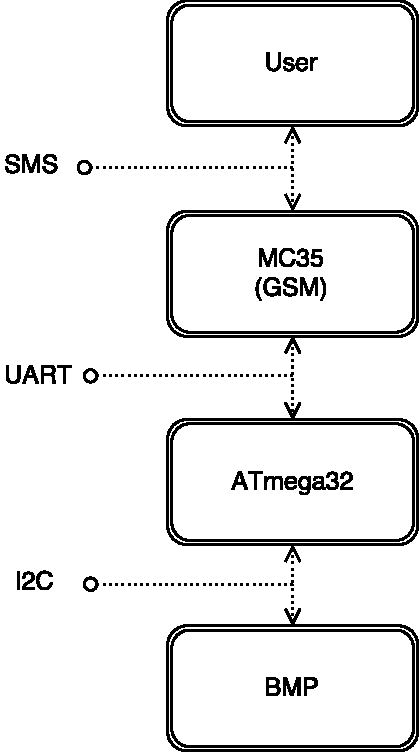
\includegraphics[width=\linewidth]{figs/blockdiagram.pdf}
	\caption{Blokdiagram for system.}
	\label{fig:blockdiagram}
\end{figure}
\vskip 0.5cm

Sekvensdiagrammet, figur~\ref{fig:seq-getdata} viser det overordnede flow igennem programmet fra at en bruger har sendt en sms, til at samme bruger får den ønskede måling tilbage.

\begin{figure}[h]
	\centering
	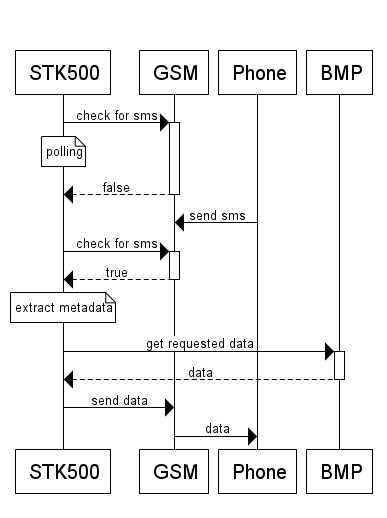
\includegraphics[width=0.56\linewidth]{figs/seq-getdata.png}
	\caption{Sekvensdiagram for hentning af data.}
	\label{fig:seq-getdata}
\end{figure}
